\documentclass{article}
\usepackage{cmap}
\usepackage[utf8]{inputenc}
\usepackage[english,ukrainian]{babel}
\usepackage{graphicx}
\usepackage{geometry}
\usepackage{listings}
\usepackage{float}
\usepackage{amsmath}
\usepackage{subfig}
\usepackage{xcolor}
\geometry{
	a4paper,
	left=20mm,
	right=20mm,
	top=15mm,
	bottom=15mm,
}
\lstset{
	tabsize=4,
	keepspaces,
	showstringspaces=false,
	escapeinside={(*@}{@*)},
}
\graphicspath{ {./pictures} }
\setlength{\parindent}{4em}

\newcommand\subject{Архітектура комп'ютера}
\newcommand\lecturer{доцент кафедри ПЗ\\Крук О.Г.}
\newcommand\teacher{доцент кафедри ПЗ\\Крук О.Г.}
\newcommand\mygroup{ПЗ-22}
\newcommand\lab{5}
\newcommand\theme{Складення та відлагодження циклічної програми мовою асемблера мікропроцесорів х86 для Windows}
\newcommand\purpose{Ознайомитись на прикладі циклічної програми з основними командами асемблера; розвинути навики складання програми з вкладеними циклами; відтранслювати і виконати в режимі відлагодження програму, складену відповідно до свого варіанту; перевірити виконання тесту}

\begin{document}
\begin{normalsize}
	\begin{titlepage}
		\thispagestyle{empty}
		\begin{center}
			\textbf{МІНІСТЕРСТВО ОСВІТИ І НАУКИ УКРАЇНИ\\
				НАЦІОНАЛЬНИЙ УНІВЕРСИТЕТ "ЛЬВІВСЬКА ПОЛІТЕХНІКА"}
		\end{center}
		\begin{flushright}
			\textbf{ІКНІ}\\
			Кафедра \textbf{ПЗ}
		\end{flushright}
		\vspace{200pt}
		\begin{center}
			\textbf{ЗВІТ}\\
			\vspace{10pt}
			до лабораторної роботи № \lab\\
			\textbf{на тему}: “\textit{\theme}”\\
			\textbf{з дисципліни}: “\subject”
		\end{center}
		\vspace{112pt}
		\begin{flushright}
			
			\textbf{Лектор}:\\
			\lecturer\\
			\vspace{28pt}
			\textbf{Виконав}:\\
			
			студент групи \mygroup\\
			Коваленко Д.М.\\
			\vspace{28pt}
			\textbf{Прийняв}:\\
			
			\teacher\\
			
			\vspace{28pt}
			«\rule{1cm}{0.15mm}» \rule{1.5cm}{0.15mm} 2022 р.\\
			$\sum$ = \rule{1cm}{0.15mm}……………\\
			
		\end{flushright}
		\vspace{\fill}
		\begin{center}
			\textbf{Львів — 2022}
		\end{center}
	\end{titlepage}
		
	\begin{description}
		\item[Тема.] \theme.
		\item[Мета.] \purpose.
	\end{description}

	\section*{Індивідуальне завдання}
	\begin{figure}[H]
		\centering
		
\includegraphics[scale=0.6]{v}
	\end{figure}
	
	\section*{Хід роботи}
	\section*{Програма 1}
	\begin{figure}[H]
		\centering
		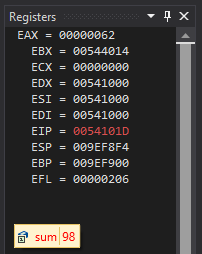
\includegraphics[scale=1]{1}
		\caption{Стан регістрів та змінної $sum$ після виконання програми}
	\end{figure}
	\begin{gather}
		17+3-51+242-113=98_{10}=62_{16}\nonumber
	\end{gather}

	\section*{Програма 2}
	\begin{gather}
		\text{3 рядок: }a= -81,-78,-82,-39,-90,-78, 24\nonumber\\
		\text{5 рядок: }b=56,-19,-86, 34,-83,-99,-31\nonumber\\
		\text{Скалярний добуток:}\sum_{i=1}^{7}a_ib_i=-81\cdot56-78\cdot(-19)-82\cdot(-86)-39\cdot34-90\cdot(-83)-78\cdot(-99)+24\cdot(-31)=\nonumber\\=-4536+1482+7052-1326+7470+7722-744=17120\nonumber
	\end{gather}

	\begin{figure}[H]
		\centering
		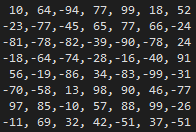
\includegraphics[scale=1]{2}
		\caption{Двовимірний масив, що необхідно було транспонувати}
	\end{figure}

	\begin{figure}[H]
		\centering
		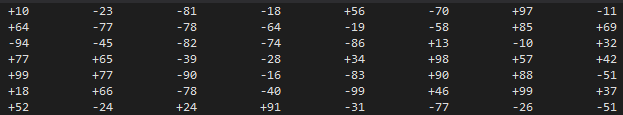
\includegraphics[scale=0.7]{3}
		\caption{Відображення транспонованого масиву у пам'яті}
	\end{figure}

	\begin{figure}[H]
		\centering
		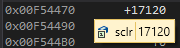
\includegraphics[scale=1]{4}
		\caption{Результат обчислення скалярного добутку}
	\end{figure}

	\begin{gather}
		\text{Стовпець 3:} -94,-45,-82,-74,86,13,-10,95\nonumber\\
		\text{Кількість елементів, що задовільняють умову: } 6\nonumber\\
		\text{Сума елементів, що задовільняють умову: } -114\nonumber		
	\end{gather}

	\begin{figure}[H]
		\centering
		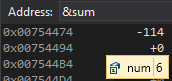
\includegraphics[scale=1]{5}
		\caption{Результат знаходження кількості та суми за заданою умовою}
	\end{figure}

	\subsection*{Код програми 2}
	\begin{lstlisting}[language={[x86masm]Assembler}]
.586P 
.MODEL FLAT, STDCALL 

_DATA SEGMENT 
tmp      DD 0
col      DD 7
row      DD 8
arr      DD  10, 64,-94, 77, 99, 18, 52
		 DD -23,-77,-45, 65, 77, 66,-24
		 DD -81,-78,-82,-39,-90,-78, 24
		 DD -18,-64,-74,-28,-16,-40, 91
		 DD  56,-19, 86, 34,-83,-99,-31
	 	 DD -70,-58, 13, 98, 90, 46,-77
	 	 DD  97, 85,-10, 57, 88, 99,-26
		 DD -11, 69, 95, 42,-51, 37,-51
res      DD 224 DUP(?)
sclr     DD 0
num      DD 0
sum      DD 0
_DATA ENDS 

_TEXT SEGMENT 
START:

T1:
	lea ECX, arr
	lea EDX, res
	mov EBX, 0

L1: 
	mov EAX, 0

L2:     
	lea ECX, arr 
	lea EDX, res 
	
	mov tmp, EAX 
	push EAX
	push EDX
	push ECX
	mov EAX, tmp
	mul col
	add EAX, EBX
	push EBX
	mov EBX, 4
	mul EBX
	pop EBX
	pop ECX
	add ECX, EAX
	pop EDX
	pop EAX
	
	mov tmp, EAX
	push EAX
	push ECX
	push EDX
	mov EAX, EBX
	mul row
	add EAX, tmp
	push EBX
	mov EBX, 4
	mul EBX
	pop EBX
	pop EDX
	add EDX, EAX
	pop ECX
	pop EAX
	
	push EAX 
	mov EAX, [ECX]
	mov [EDX], EAX
	pop EAX
	
	inc EAX  
	cmp EAX, row
	jl L2
	
	inc EBX   
	cmp EBX, col
	jl L1

T2:
	lea EDX, arr 
	add EDX, 56
	mov EBX, EDX
	
	lea EDX, arr 
	add EDX, 112
	mov ECX, EDX
	mov EDX, 0

L3:    
	mov EAX, [EBX] 
	push EDX
	mov EDX, [ECX]
	imul EDX
	pop EDX
	add sclr, EAX
	
	add EBX, 4
	add ECX, 4
	
	inc EDX   
	cmp EDX, col
	jl L3

T3:     
	lea EAX, arr  
	add EAX, 8
	mov EDX, 0

L4:
	cmp EDX, row 
	jge T4
	
	inc EDX
	
	mov EBX, [EAX] 
	cmp EBX, -29
	jle COUNT
	cmp EBX, 83 
	jge COUNT
	add EAX, 28
	jmp L4

COUNT:
	inc num
	add EAX, 28
	jmp L4

T4:
	lea EAX, arr  
	add EAX, 8
	mov EDX, 0

L5:
	cmp EDX, row  
	jge DONE
	
	inc EDX
	
	mov EBX, [EAX]  
	cmp EBX, -29
	jle SUMUP
	cmp EBX, 83 
	jge SUMUP
	add EAX, 28
	jmp L5

SUMUP:
	add sum, EBX
	add EAX, 28
	jmp L5

DONE:

RET
_TEXT ENDS 
END START
	\end{lstlisting}

	\section*{Висновки}
	Під час виконання лабораторної роботи я ознайомився на прикладі циклічної програми з основними командами асемблера; розвинув навики складання програми з вкладеними циклами; відтранслював і виконати в режимі відлагодження програму, складену відповідно до свого варіанту; перевірив виконання тесту.
	    
\end{normalsize}
\end{document}
